%************************************************
\chapter{The Kerr-Schild coordinate system}\label{ch:introduction}
%************************************************
The Kerr metric defined originally in \gls{BL} coordinates \cite{boyer2004maximal} has multiple singular points. These singular points in the metric are associated only to the election of the coordinate system and are not true spacetime singularities. The existence of this kind of ''coordinate singularities'' prevent us to obtain continuous geodesic equations  when crossing the horizons that this false singular points define. To get rid of this problem, we will transform the metric from \gls{BL} coordinates to another coordinate system called \gls{KS} coordinate system in which the metric has only the true spacetime singularity located at $r=0$ (in \gls{BL} coordinates). In addition, the new coordinate system will reveal some hidden features in the Kerr spacetime that there are only clear when the metric is expressed in this way. This will allow us to analyze some of the geodesic movements that can only be correctly analyzed is this system, wherein the true form of singularity is revealed. To achieve this coordinate transform we will need to perform a previous transform into the \gls{EF} coordinate system in order to finally express the metric in \gls{KS} coordinates.


\section{Metric in Eddington-Finkenstain coordinates}
In this section we are going to transform the Kerr metric from \gls{BL} coordinates into \gls{EF} keeping the sign of the future causal vector that defines this coordinates.
\begin{lemma}\label{lemma:BLtoEF}
 The Kerr metric defined on \gls{BL} coordinates
 \begin{align*}
 ds^2&=-d\bar{t}^2+ \Sigma \left(\frac{dr^2}{\Delta}+d\theta^2 \right)+(r^2+a^2)\sin^2{(\theta)} d\bar{\phi}^2\\
 &+\frac{2 M r}{\Sigma}(a \sin^2{(\theta)} d \bar{\phi} -d\bar{t})^2
\end{align*}
once expressed in \gls{EF} coordinates takes the form
\begin{equation*}
\begin{aligned}
 ds^2=&-dt^2+dr^2+\Sigma d\theta^2+(r^2+a^2) \sin^2{(\theta)} d\phi^2+2\sigma a \sin^2{(\theta)} dr d\phi\\
 &+\frac{2M r}{\Sigma}(-\sigma dt+ dr-\sigma a \sin^2{(\theta)} d\phi)^2,
 \end{aligned}
\end{equation*}
\end{lemma}
\begin{Proof}
We start with the expression of the metric in \gls{BL} coordinates
\begin{align}\label{eq:Kerrmetricblsimpl}
 ds^2&=-d\bar{t}^2+ \Sigma \left(\frac{dr^2}{\Delta}+d\theta^2 \right)+(r^2+a^2)\sin^2{(\theta)} d\bar{\phi}^2\\
 &+\frac{2 M r}{\Sigma}(a \sin^2{(\theta)} d \bar{\phi} -d\bar{t})^2
\end{align}
where $\Delta=r^2-2 M r+a^2$ and $\Sigma=r^2+a^2 \cos^2{(\theta)}$. The \gls{EF} coordinates are defined to be the coordinate system adapted to the geodesic of the null vectors
\begin{equation}
 l^\mu=\left( \frac{d\bar{t}}{d\tau},\frac{dr}{d\tau},\frac{d\theta}{d\tau},\frac{d\bar{\phi}}{d\tau} \right)=\left( \frac{r^2+a^2}{\Delta},\sigma,0,\frac{a}{\Delta} \right),
\end{equation}
where $\sigma=1$ correspond to the outgoing coordinate system and $\sigma=-1$ correspond to the ingoing coordinate system. Let us parametrize the geodesic in terms of $r$ as
\begin{equation}
 \frac{d\bar{t}}{dr}=\sigma \frac{r^2+a^2}{\Delta} \quad \quad  \frac{d\bar{\phi}}{dr}=\sigma \frac{a}{\Delta}.
\end{equation}
We want these geodesics to be coordinate lines of our new system; thus, one of our coordinates is r, while the others are quantities which are constant along each geodesic belonging to the
family. One of these is $\theta$; the remaining two coordinates are given by
\begin{align}
 v &\equiv \bar{t} - \sigma T(r),\\
\phi &\equiv \bar{\phi} - \sigma \Phi(r),
\end{align}
where $\Phi(r)$ and $T(r)$ are chosen to fulfill
\begin{align}
 \frac{dT}{dr}&=\frac{r^2+a^2}{\Delta},\\
 \frac{d\Phi}{dr}&=\frac{a}{\Delta}.
\end{align}
Therefore, along this family of geodesics we have that
\begin{equation}
 \frac{dv}{dr}=\frac{d\phi}{dr}=0,
\end{equation}
and the tangent vector in this new coordinate system is simply $l^\mu=\left( 0,\sigma,0,0 \right)$. We can now compute the metric tensor in \gls{EF} coordinate system. We have that
\begin{align}
 dv&=d\bar{t}- \sigma \frac{r^2+a^2}{\Delta} dr, \label{eq:Kerrcoordtrans1} \\
 d\phi&=d\bar{\phi}- \sigma \frac{a}{\Delta}. \label{eq:Kerrcoordtrans2}\\
\end{align}
Then, we can compute the following relations
\begin{align}
 -d\bar{t}^2&=-dv^2-\frac{(r^2+a^2)^2}{\Delta^2} dr^2 \nonumber\\
 &-\sigma 2 \frac{r^2+a^2}{\Delta} dv dr,\\
 (r^2+a^2) \sin^2{(\theta)} d\bar{\phi}^2&=(r^2+a^2)\sin^2{(\theta)} d\phi \nonumber\\
 &+(r^2+a^2)\frac{a^2}{\Delta^2} \sin^2{(\theta)} dr^2 \nonumber\\
 &+ \sigma 2(r^2+a^2)\sin^2{(\theta)}\frac{a}{\Delta}  dr d\phi,\\
 \frac{2M r}{\Sigma}(dt-a \sin^2{(\theta)} d\bar\phi)^2&= \frac{2M r}{\Sigma} dv^2 +\frac{2M r}{\Sigma} a^2 \sin{\theta}^4 d\phi^2 \nonumber\\
 &+ \frac{2M r \Sigma}{\Delta^2} dr^2 -\frac{4 a  M r \sigma  \sin ^2(\theta )}{\Delta } dr d\phi \nonumber\\
 &-\frac{4 a  M r \sin ^2(\theta )}{\Sigma } dv d\phi\nonumber\\
 &+\frac{4  M r \sigma }{\Delta } dr dv.
\end{align}
Collecting terms in $dr,dv,d\phi,d\theta$ we  can rewrite the metric tensor as
\begin{equation}
 \begin{aligned}
ds^2&=-\left( 1- \frac{2 M r}{\Sigma} \right) dv^2- 2\sigma dvdr+\Sigma d\theta^2\\
&+\frac{(r^2+a^2)^2-\Delta a^2 \sin^2{(\theta)}}{\Sigma}\sin^2{(\theta)} d\phi^2\\
&+2 \sigma a \sin^2{(\theta)}  dr d\bar\phi-\frac{4 m r a}{\Sigma} \sin^2{(\theta)} dv d\phi
 \end{aligned}
\end{equation}
Which can be rearrange into
\begin{equation}
\begin{aligned}
ds^2&=-dv^2-2 \sigma dv dr +\Sigma d\theta^2+(r^2+a^2) \sin^2{(\theta)} d\phi^2 \\
&+ 2 \sigma a \sin^2{(\theta)} dr d\phi + \frac{2 M r}{\Sigma} (-dv +a \sin^2{(\theta)} d\phi)^2.
\end{aligned}
\end{equation}
We can now define a explicit time coordinate (which we will name $t$ but does not coincide with the time coordinate of \gls{BL} coordinates)
\begin{equation}\label{eq:timeeq2}
 t \equiv  v + \sigma r
\end{equation}
so that the metric becomes
\begin{equation}
\begin{aligned}
 ds^2=&-dt^2+dr^2+\Sigma d\theta^2+(r^2+a^2) \sin^2{(\theta)} d\phi^2+2\sigma a \sin^2{(\theta)} dr d\phi\\
 &+\frac{2M r}{\Sigma}(-dt+\sigma dr+a \sin^2{(\theta)} d\phi)^2,
 \end{aligned}
\end{equation}
Which is equivalent to
\begin{equation}\label{eq:KerrmetricKerr}
\begin{aligned}
 ds^2=&-dt^2+dr^2+\Sigma d\theta^2+(r^2+a^2) \sin^2{(\theta)} d\phi^2+2\sigma a \sin^2{(\theta)} dr d\phi\\
 &+\frac{2M r}{\Sigma}(-\sigma dt+ dr+\sigma a \sin^2{(\theta)} d\phi)^2,
 \end{aligned}
\end{equation}\end{Proof}

\section{Metric in Kerr-Schild form}

Now that we have the Kerr metric expressed in \gls{EF} for both time orientations (encoded in the sign of $\sigma$), we are ready to transform the metric into its final form in \gls{KS} coordinates. once we have the metric in this coordinates we will proceed to analyze the features that are only revealed in this coordinate system.

\subsection{Displaying the metric in Kerr-Schild coordinates}

\begin{lemma}
 The Kerr metric defined on \gls{BL} coordinates
 \begin{align*}
 ds^2&=-d\bar{t}^2+ \Sigma \left(\frac{dr^2}{\Delta}+d\theta^2 \right)+(r^2+a^2)\sin^2{(\theta)} d\bar{\phi}^2\\
 &+\frac{2 M r}{\Sigma}(a \sin^2{(\theta)} d \bar{\phi} -d\bar{t})^2
\end{align*}
once expressed in \gls{KS} coordinates takes the form
\begin{equation*}
 g=\eta + h K \otimes K,
\end{equation*}
where $\eta$ is the Minkowsky metric and
\begin{align*}
 f&=\frac{2 M r^3}{r^4+a^2 z^2}, \nonumber \\
 K&=-\sigma dt + \frac{r(x dx+y dy)}{r^2+a^2} + \frac{a(x dy-y dx)}{r^2+a^2}+\frac{z dz}{r}. \nonumber
\end{align*}
\end{lemma}
\begin{Proof}
By the use of  \cref{lemma:BLtoEF} we can start with the expression of the metric in \gls{EF} coordinates. The goal is transform the metric
\begin{equation}
\begin{aligned}
 ds^2=&-dt^2+dr^2+\Sigma d\theta^2+(r^2+a^2) \sin^2{(\theta)} d\phi^2+2\sigma a \sin^2{(\theta)} dr d\phi\\
 &+\frac{2M r}{\Sigma}(-\sigma dt+ dr+\sigma a \sin^2{(\theta)} d\phi)^2,
 \end{aligned}
\end{equation}
into \gls{KS} coordinates. The \gls{KS} \cite{kerr1965new} coordinates $(T,x,y,z)$ are defined by
\begin{align}
 x&=\sqrt{r^2+a^2} \sin{(\theta)} \cos\left( \sigma\phi- \arctan{\frac{a}{r}} \right), \label{eq:KSCoor1}\\
 y&=\sqrt{r^2+a^2} \sin{(\theta)} \sin \left( \sigma\phi- \arctan{\frac{a}{r}} \right), \label{eq:KSCoor2}\\
 z&=r\cos{\theta} \label{eq:KSCoor3}.
\end{align}
From defining $\beta=\arctan{\frac{a}{r}}$  we have
\begin{equation}
 r^2 \sin{\beta}^2=a^2 \cos{\beta}^2,
\end{equation}
thus
\begin{align}
 r^2&=(r^2+a^2)\cos{\beta}^2, \label{eq:KSrelation1} \\
 a^2&=(r^2+a^2)\sin{\beta}^2. \label{eq:KSrelation2}
\end{align}
We can rewrite \cref{eq:KSCoor1,eq:KSCoor2} as
\begin{align}
x&=\sqrt{r^2+a^2} \sin{\theta} ( \cos{\beta} \cos{(\sigma \phi)}+ \sin{\beta} \sin{(\sigma\phi)}), \\
y&=\sqrt{r^2+a^2} \sin{\theta} ( \cos{\beta} \sin{(\sigma \phi)}- \sin{\beta} \cos{(\sigma\phi)}), \\
x&=r\cos{\theta},
\end{align}
and substituting \cref{eq:KSrelation1,eq:KSrelation2} into this relations it follows that
\begin{align}
 x&= \sin{\theta} ( r \cos{(\sigma\phi)}+ a \sin{(\sigma\phi)}) \label{eq:KSCoor1fina}, \\
 y&= \sin{\theta} ( r \sin{(\sigma\phi)}- a \cos{(\sigma\phi)}) \label{eq:KSCoor2fina}, \\
 z&=r\cos{\theta} \label{eq:KSCoor3fina}.
\end{align}
Differentiating this relations we obtain that
\begin{align}
dx&=d\theta \cos (\theta ) (a \sin ( \sigma\phi  )+r  \cos ( \sigma\phi  ))+dr  \sin (\theta ) \cos (\sigma\phi ) \nonumber \\
&+d\phi \sin (\theta ) (a \sigma  \cos (\sigma  \phi )-r \sigma  \sin (\sigma  \phi )) \label{eq:KSdifferentials1}\\
dy&=d\phi \sin (\theta ) (a \sigma  \sin (\sigma  \phi )+r \sigma  \cos (\sigma  \phi ))+dr  \sin (\theta ) \sin (\sigma \phi )\nonumber \\
&+d\theta \cos (\theta ) (r  \sin (\sigma \phi )-a \cos (\sigma \phi ))\label{eq:KSdifferentials2} \\
dz&=dr\cos (\theta )-d\theta r \sin (\theta )\label{eq:KSdifferentials3}
\end{align}
We can relate the Minkowsky metric in \gls{KS} coordinates with the \gls{EF} coordinates as
\begin{equation}
\begin{aligned}
 dx^2+dy^2+dz^2-dt^2&= dr^2 + (r^2 +a^2 \cos^2{(\theta)} ) d\theta^2\\
 &+ (r^2+a^2)\sin^2{(\theta)} d\phi^2+2 \sigma \sin^2{(\theta)} a dr d\phi -dt^2.
\end{aligned}
\end{equation}
Comparing this with the metric \cref{eq:KerrmetricKerr} we realize that the Kerr metric can be written as
\begin{equation}
\begin{aligned}
 &dx^2+dy^2+dz^2-dt^2+\frac{2 M r}{r^2+\cos^2{(\theta)}} (-\sigma dt+ dr+\sigma a \sin^2{(\theta)} d\phi)^2\\
 &=dx^2+dy^2+dz^2-dt^2+\frac{2 M r^3}{r^4+a^2 z^2} (-\sigma dt+ dr+\sigma a \sin^2{(\theta)} d\phi)^2
 \end{aligned}
\end{equation}
To complete the coordinate transformation we have to express the one-form $K=-\sigma dt+dr+\sigma a \sin^2{(\theta)} d\phi$ into Kerr-Schild coordinates. To achieve that we will prove that
\begin{equation}
 -\sigma dt+dr+ \sigma a \sin^2{(\theta)} d\phi= dt + \frac{r(x dx+y dy)}{r^2+a^2} + \frac{a(x dy-y dx)}{r^2+a^2}+\frac{z dz}{r}.
\end{equation}
We start expressing first \cref{eq:KSdifferentials1,eq:KSdifferentials2,eq:KSdifferentials3} as
\begin{align}
 dx&=\frac{\cos{(\theta)}}{\sin{(\theta)}} x d\theta +\sin( \theta) \cos{(\sigma \phi)} dr-\sigma y d\phi,\\
  dy&=\frac{\cos{(\theta)}}{\sin{(\theta)}} y d\theta +\sin( \theta) \sin{(\sigma \phi)} dr+\sigma x d\phi,\\
  dz&=-r \sin( \theta) d\theta +\cos( \theta) dr.
\end{align}
From this relations we have
\begin{align}
x dx+ y dy &= \frac{\cos{(\theta)}}{\sin{(\theta)}} (x^2+y^2) d\theta + \sin( \theta) (x cos{(\sigma \phi)} +y \sin{(\sigma \phi)}) dr \nonumber\\
&=\sin( \theta) \cos( \theta) (r^2+a^2) d\theta+\sin^2{(\theta)} r dr, \\
xdy-y dx &= \sigma (x^2+y^2) d\phi-\sin{(\theta)} (y \cos{(\sigma \phi)} - x \sin{(\sigma \phi)}) dr \nonumber\\
&=\sigma (r^2+a^2) \sin^2{(\theta)} d\phi +\sin^2{(\theta)} a dr,\\
z dz &= -r^2 \sin{(\theta)} \cos{(\theta)} d\theta+r \cos^2{(\theta)} dr.
\end{align}
then
\begin{equation}
\begin{aligned}
&\frac{r(x dx+y dy)}{r^2+a^2} + \frac{a(x dy-y dx)}{r^2+a^2}+\frac{z dz}{r}\\
&=(r \sin( \theta) \cos( \theta) d\theta + \frac{r^2}{r^2+a^2} \sin^2{(\theta)} dr)\\
&+(\sigma a \sin^2{(\theta)} d\phi + \frac{a^2}{r^2+a^2} \sin^2{(\theta)} dr)\\
&+(-r \sin{(\theta)} \cos{(\theta)} d\theta+ \cos^2{(\theta)} dr)\\
&=dr+\sigma a \sin^2{(\theta)} .\end{aligned}
\end{equation}
Therefore, the Kerr metric in \gls{KS} coordinates can be written as
\begin{equation}\label{eq:metricinKS}
 g=\eta + h K \otimes K,
\end{equation}
where $\eta$ is the Minkowsky metric and
\begin{align}
 f&=\frac{2 M r^3}{r^4+a^2 z^2}, \nonumber \\
 K&=-\sigma dt + \frac{r(x dx+y dy)}{r^2+a^2} + \frac{a(x dy-y dx)}{r^2+a^2}+\frac{z dz}{r}. \nonumber
\end{align}
\end{Proof}

\subsection{Surface embedding into Kerr-Schild coordinates}
  \begin{figure}   
\begin{center}
 \centerline{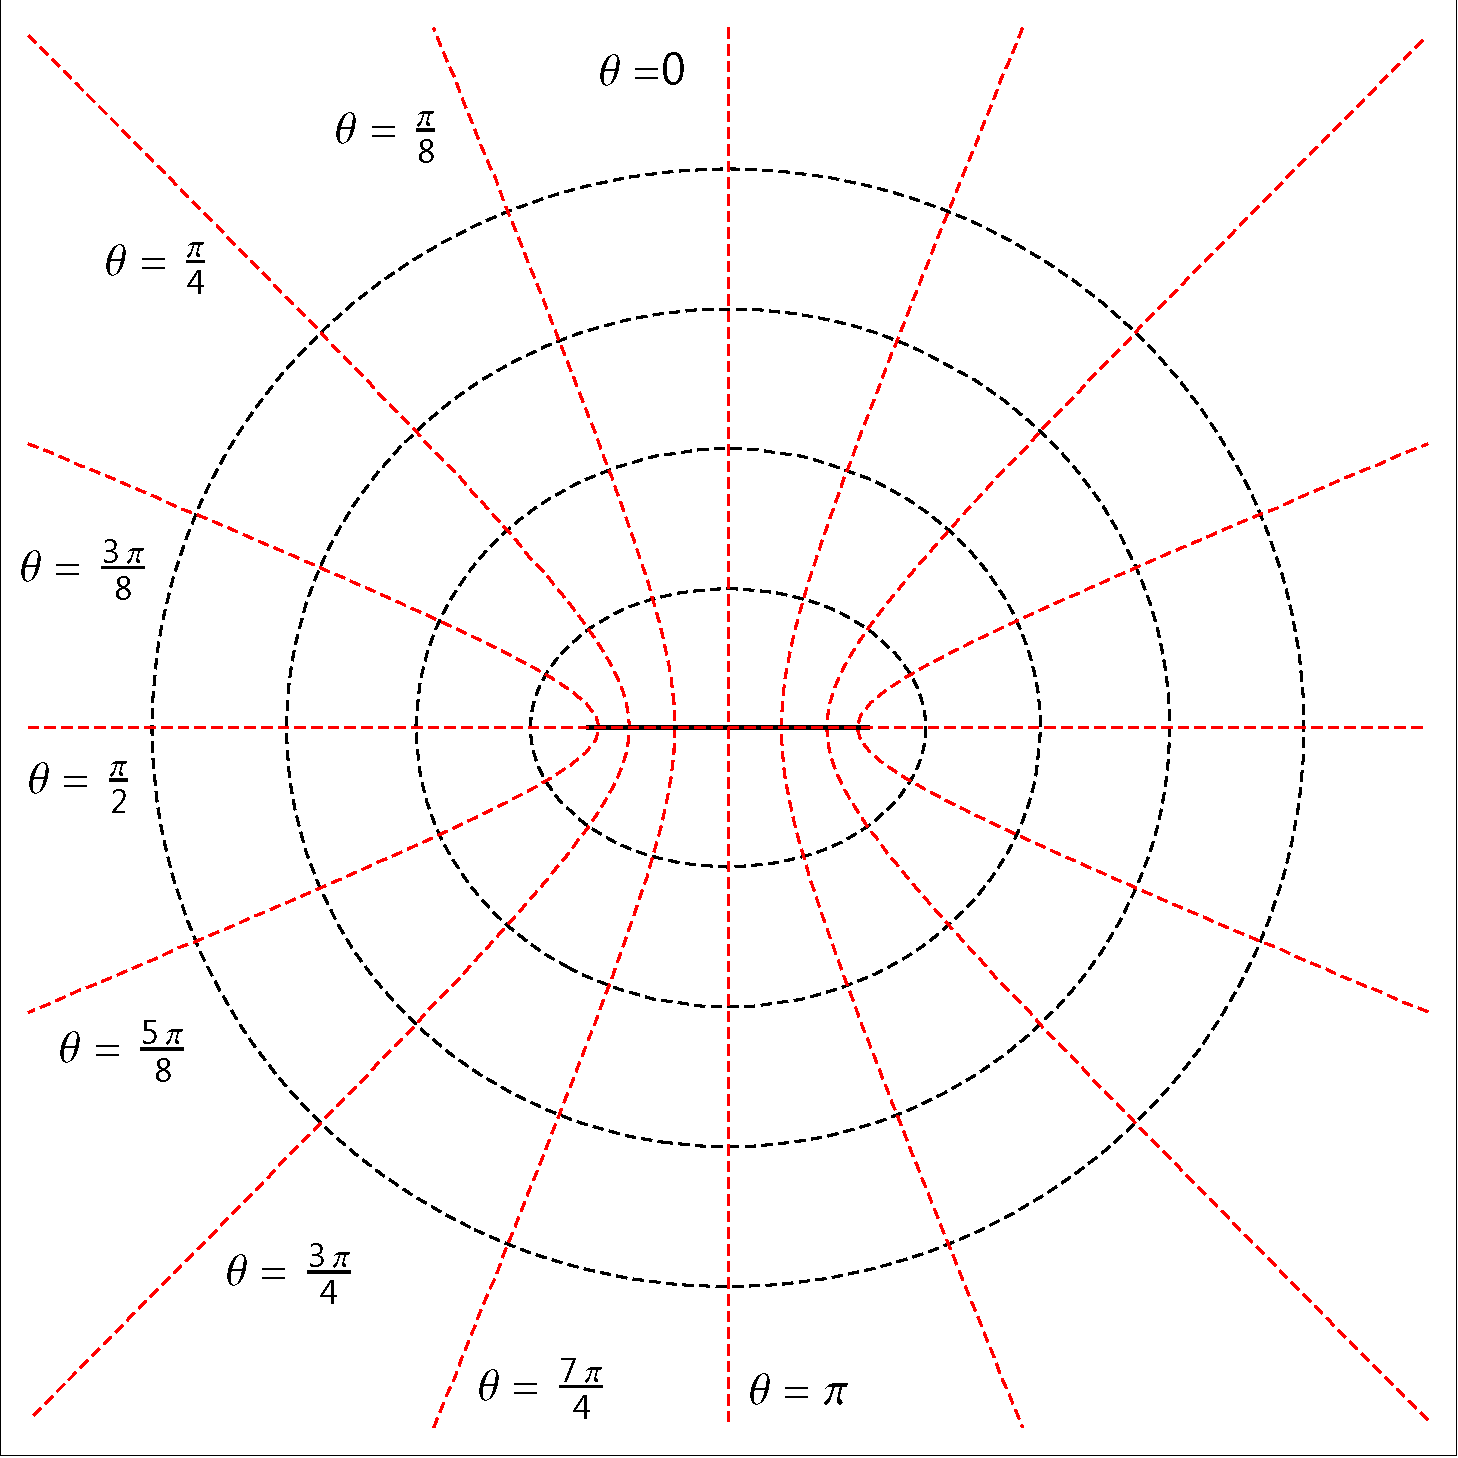
\includegraphics[width=.7\textwidth]{img/Chapter1/Surfaces.pdf}}
 \end{center}
 \caption{Surfaces with constant $r$ (black ellipsoids) and constant $\theta$ (red half\- -hyperboloids) in the Kerr spacetime.}
 \label{fig:Constantsurfaces}
\end{figure} 
We are now able to see how the different surfaces are embedded in the Kerr-Schild version of the Kerr spacetime. Let's start with the \gls{BL}-constant-coordinate surfaces. Notice that from \cref{eq:KSCoor1fina,eq:KSCoor2fina,eq:KSCoor3fina} it follows that
\begin{align}
 x^2+y^2&=(a^2+r^2) \sin^2{(\theta)},\\
 z^2&=r^2 \cos^2(\theta),
\end{align}
thus
\begin{align}
 1&=\frac{x^2+y^2}{r^2+a^2}+\frac{z^2}{r^2} \label{eq:rdefinition},\\
 1&=\frac{x^2+y^2}{a^2 \sin^2(\theta)}-\frac{z^2}{a^2 \cos^2(\theta)}.
\end{align}
The first equation serves as implicit definition of the function $r=r(x,y,z)$ and tell us that the surfaces with constant $r$ are ellipsoids while the second equation shows that the surfaces with constant $\theta$ are half-hyperboloids. This surfaces are displayed in \vref{fig:Constantsurfaces}.
A helpful diagram of the horizons and singularities can be found in \vref{fig:Horizons,fig:ergo2}
 \begin{figure}[ht!] 
\begin{center}
 \centerline{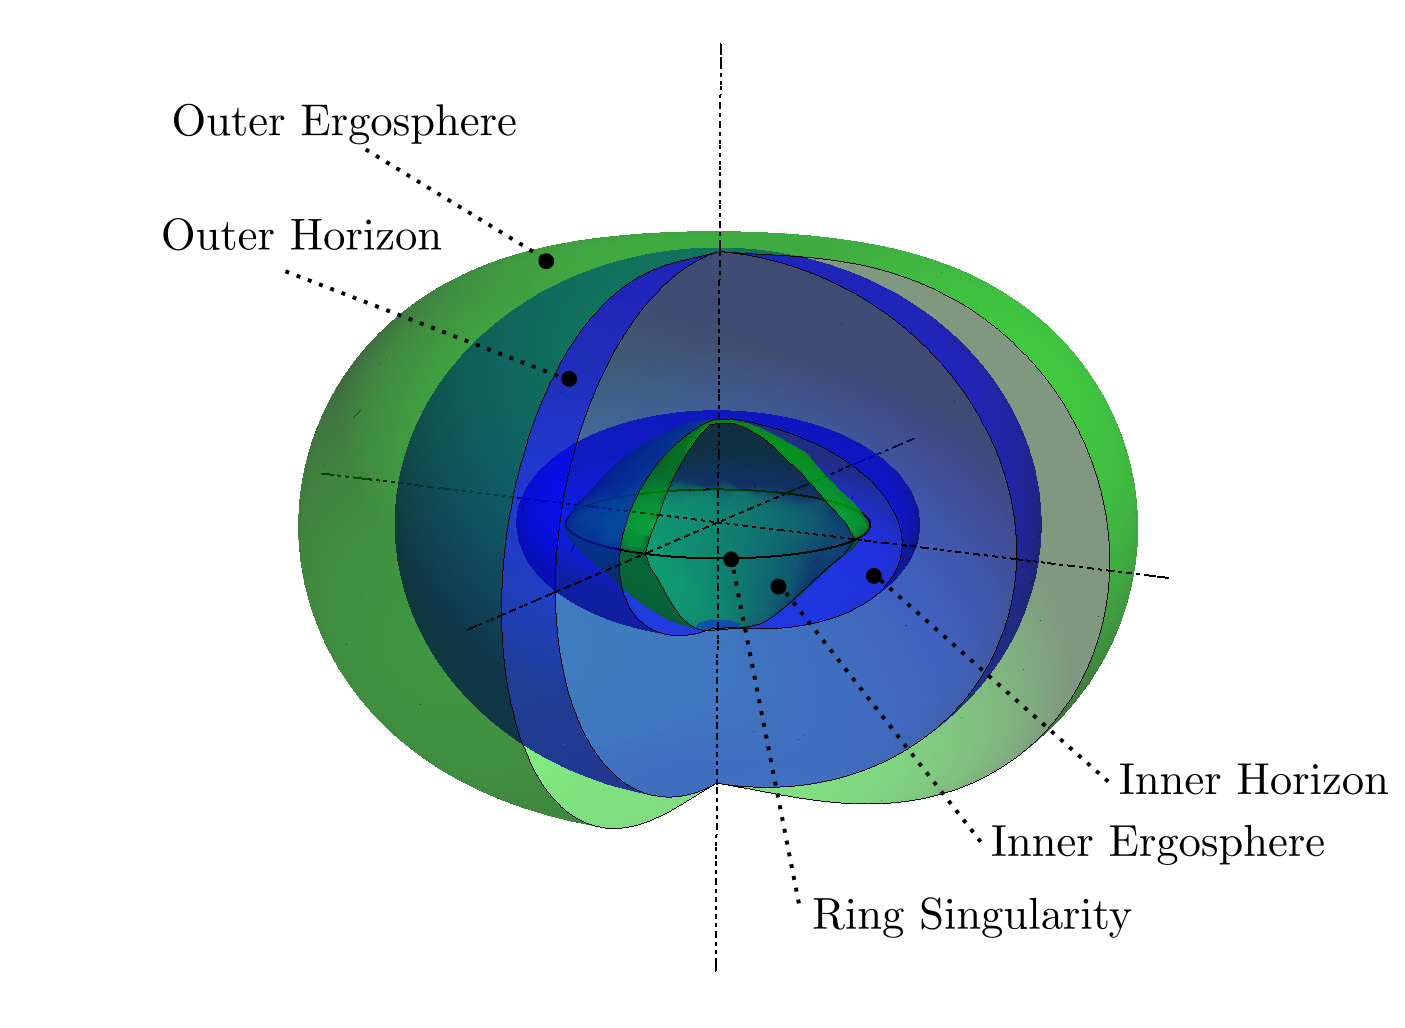
\includegraphics[width=0.9\textwidth]{img/Chapter1/Horizons.png}}
 \end{center}
 \caption{Schematic location of the horizons, ergosurfaces, and curvature singularity in the Kerr spacetime. For simplicity $M=1$ and $a=0.9$ is chosen.}
 \label{fig:Horizons}
\end{figure}
  \begin{figure}[htp!]  
\begin{center}
 \centerline{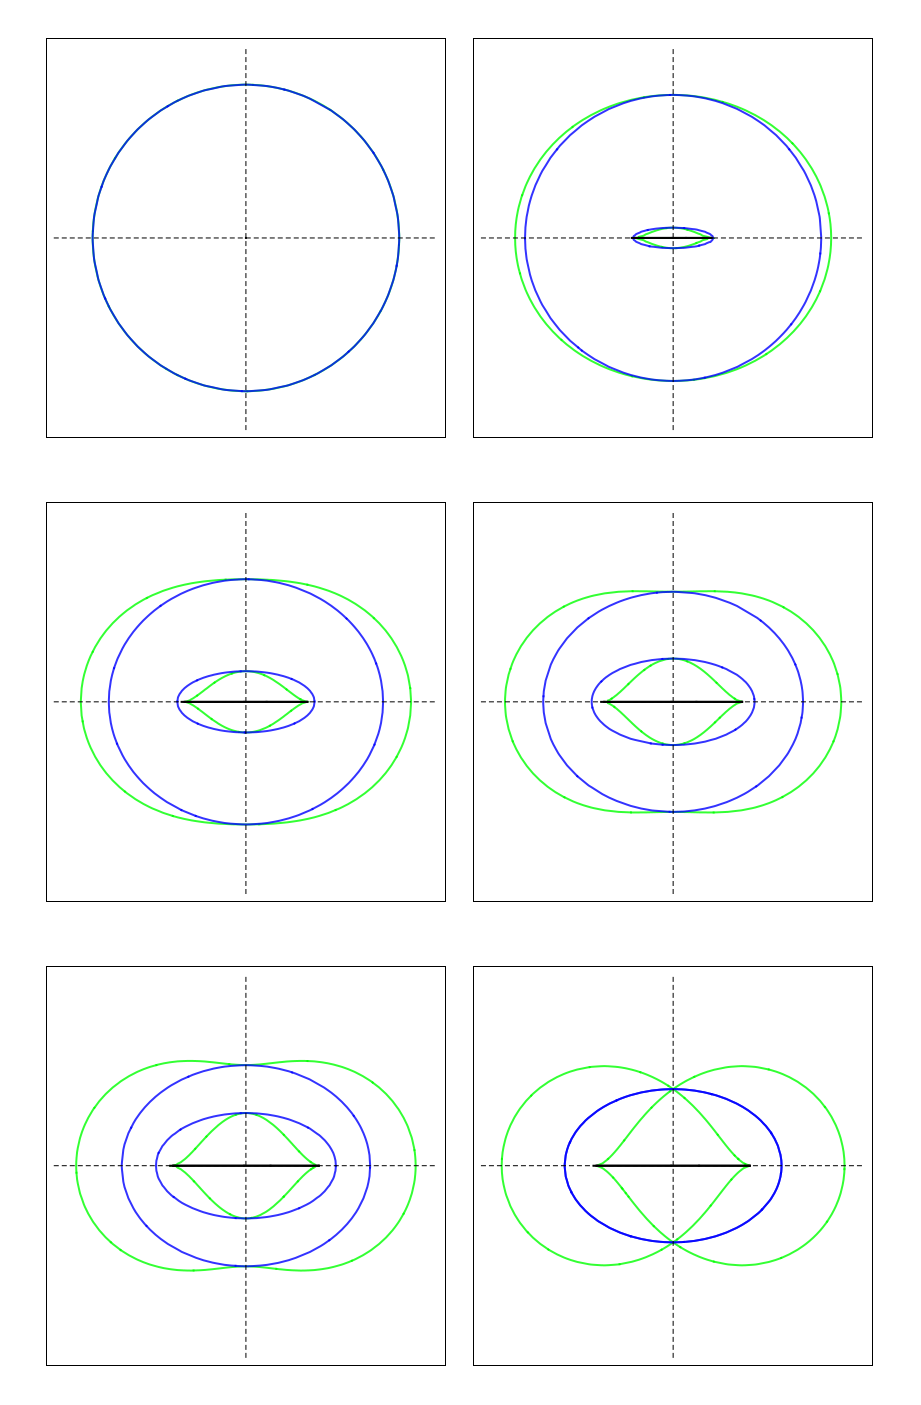
\includegraphics[width=0.95\textwidth]{img/Chapter1/erg2.png}}
 \end{center}
 \vspace{-1.5cm}
 \caption{Schematic location of the horizons, ergosurfaces, and curvature singularity in the side view of the Kerr-Schild Spacetime as a function of the parameter $a$. The images correspond to (from left to right and from top to bottom) $a=0$,$a=0.5$,$a=0.8$,$a=0.9$,$a=0.95$,$a=1$- The green surfaces are the outer and inner ergosurfaces and the blue curves represent the inner and outer horizon. The ring singularity is represented as the black curve while the black dashed curves are the $z$ and $y$ Kerr-Schild axes. For simplicity $M=1$ is chosen.}
 \label{fig:ergo2}
\end{figure} 
Now that we know how the \gls{BL}-constant-coordinate surfaces look like in the \gls{KS} version of the Kerr spacetime, we will proceed to analyze the singularity surfaces. Notice that the metric \ref{eq:metricinKS} is only singular at $x^2+y^2=a^2$ and therefore all the remaining singularities that we find in \gls{BL} coordinates or \gls{EF} coordinates are gone. The remaining singularity is the \textit{True} spacetime singularity and once embedded in the \gls{KS} version of the Kerr spacetime the ring shape is revealed. Transforming the solutions to the singularity equations ($\Delta=r^2-2 M r+a^2=0$ and $\Sigma=r^2+a^2 \cos^2{(\theta)}=0$), which gives the horizons and the spacetime singularity, and the solution to the points where $g_{tt}$ changes sign ($g_tt=-1+\frac{2Mr}{\Sigma}=0$), which gives the ergosurfaces, to \gls{KS} coordinates we realize that the horizons and singularities of the Kerr metric in \gls{KS} coordinates are
\begin{enumerate}
 \item Spacetime singularity at $x^2+y^2=a^2$ and $z=0$,
 \item Event horizon at $r_+=M+\sqrt{m^2-a^2}$,
 \item Cauchy horizon at $r_-=M-\sqrt{m^2-a^2}$,
 \item Outer Ergosurface at $r_\text{E}^+=M+\sqrt{M^2-a^2 \frac{z^2}{r^2}}$,
  \item Inner Ergosurface at $r_\text{E}^-=M-\sqrt{M^2-a^2 \frac{z^2}{r^2}}$.
\end{enumerate}
Notice that a closer look at \cref{eq:KSCoor1,eq:KSCoor2} reveals the \gls{BL} coordinates $\{r,\phi,\theta\}$ behave like spherical coordinates for large values of $r$, which means that if we analyze the Kerr black hole far away from its center, we will tend to see the Minkowsky spacetime. When this happens we say that the metric is \textit{asymptotically flat}, i.e. the curvature in the infinity vanishes. The \gls{KS} coordinates also reveal the true nature of the Kerr singularity, despite the spacetime singularity is at $r=0$ and $\theta=\frac{\pi}{2}$ (in \gls{BL} coordinates), in \gls{KS} coordinates this reads $x^2+y^2=a^2$ and $z=0$, which is a ring in the \gls{KS} version of the Kerr spacetime. The \gls{KS} coordinates also reveal what is called \textit{the inside of the ring} which is the region $x^2+y^2<a^2$ and $z=0$. We will discuss in the next chapters the role of this inner disk in the Kerr spacetime as well as the geodesic movement in it.

\section{Conserved quantities in Kerr-Schild coordinates}

Now that we understand the metric and the bifurcation surfaces (horizons) in \gls{KS} coordinates, we have to obtain the conserved quantities in \gls{KS} coordinates. These conserved quantities comes from the existence of two Killing vectors (associated to the temporal invariance and the axisymmetric invariance) and one Killing tensor. Useful information about Killing vectors and Killing tensor can be found in \vref{Killingchapter}. To obtain the conserved quantities in the new coordinates we must get first the Killing vectors and tensors in the \gls{KS} coordinates.

\subsection{Killing vectors}
\begin{lemma}
 The Killing vectors of the Kerr metric in \gls{KS} coordinates are:
 \begin{align}
  \xi_1&=\partial_t\\
  \xi_2&=\sigma( x \partial_y - y \partial_x)
 \end{align}
\end{lemma}
 \begin{Proof}
  As the metric \cref{eq:metricinKS} does not depend on the time coordinate $t$ then $\partial_t$ is a Killing vector. To obtain the second Killing vector, is easy to notice that the metric in \gls{EF} coordinates (\cref{eq:KerrmetricKerr}) does not depend on the coordinate $\phi$ and therefore $\partial_\phi$ is a Killing vector. We only need to transform this vector into the new coordinates using the relation between \gls{KS} coordinates and \gls{EF} coordinates of \cref{eq:KSCoor1fina,eq:KSCoor2fina}, The final killing vectors are
  \begin{equation}
  \begin{aligned}
   \partial_\phi&= \frac{\partial x}{\partial \phi} \partial x + \frac{\partial x}{\partial \phi} \partial x \nonumber,\\
   &= \sin (\theta ) (a \sigma  \cos (\sigma  \phi )-r \sigma  \sin (\sigma  \phi )) \partial_x + \sin (\theta ) (a \sigma  \sin (\sigma  \phi )+r \sigma  \cos (\sigma  \phi )) \partial_y \nonumber\\
   &=\sigma( x \partial_y - y \partial_x),
   \end{aligned}
  \end{equation}
  as claimed .\end{Proof}
  
By the use of this lemma the conserved quantities defined by this Killing vectors are:
 \begin{align}
  -E &= g(\partial_t,u)\\
  \sigma L_z&= g( x \partial_y - y \partial_x,u) \label{angulardef}
 \end{align}
where $u$ is the geodesic tangent vector.
 
 \subsection{Killing tensors}

The third constant of motion was first noticed by Brandon Carter \cite{carter1987separability,carter1968global} and in his original work, it comes from a separability constant in the Hamilton-Jacobi equations once the metric is written in \gls{BL} coordinates. This third constant of motion is written in \gls{BL} coordinates as
\begin{equation}
 \mathcal{C}=(a E-\sigma L_z)^2 +p^2_{\theta} +\cos^2(\theta) \left( a^2(M^2-E^2)+\left( \frac{L_z}{\sin(\theta)} \right)^2 \right).
\end{equation}
where $L_z$ is the total angular momentum. To clarify the genesis of this third constant of motion we are going to derive it from a generalized Killing tensor.
\begin{lemma}
 The conserved quantity given by the Carter's Killing tensor in \gls{KS} coordinates is
\begin{equation}
\begin{aligned}
 \mathcal{C}&= (\sigma L_z+a E)^2 + \left( \frac{z}{r}(x p_x +y p_y)+\sqrt{r^2-z^2} p_z \right)^2 \\
 +&\frac{z^2}{r^2} \left( a^2(M^2-E^2) \right)+ \frac{L_z^2 z^2}{r^2-z^2} 
\end{aligned}
\end{equation}
\end{lemma}
\begin{Proof}
The generalized Killing equation for Killing tensor is
\begin{equation}
\nabla_{(\alpha} T_{\beta \gamma )} = 0,
\end{equation}
where $(\cdots)$ denotes symmetrization in the indexes. Is useful to use what is know as the Killing-Yano tensor, which is in some sense the ``square root'' of a Killing tensor and it is defined to fulfill
\begin{equation}\label{eq:KillingYanodef}
 T_{\alpha \beta}= F_{\alpha \gamma}F_{\beta}^\gamma,
\end{equation}
and by this definition $F_{[\alpha \gamma]}=0$ (where $[\cdots]$ denotes antisymmetrization in the indexes). Inserting this equation into the definition of the Killing tensor we get that the Killing-Yano tensor must satisfy that
\begin{equation}\label{eq:KillingYano}
 \nabla_{(\gamma} F_{\alpha) \beta} =0.
\end{equation}
Conversely, if we find a tensor $F_{\alpha \beta}$ that satisfy \cref{eq:KillingYano} we can compute the associated Killing tensor using \cref{eq:KillingYanodef}. In \cite{faridi1986precession} one can find the only independent solution of \cref{eq:KillingYano} for the Kerr metric in \gls{KS} coordinates given by
\begin{align}
 F_{\alpha \beta}&=\left(
\begin{array}{cccc}
 0 & 0 & 0 & - \sigma a \\
 0 & 0 & z & -y \\
 0 & -z & 0 & x \\
 \sigma a & y & -x & 0 \\
\end{array}
\right)\\
F^{\alpha \beta}&=\left(
\begin{array}{cccc}
 0 & 0 & 0 & \sigma a \\
 0 & 0 & z & -y \\
 0 & -z & 0 & x \\
 -\sigma a & y & -x & 0 \\
\end{array}
\right)
\end{align}
the quantity $T_{\alpha \beta}= F_{\alpha \gamma}F_{\beta}^\gamma$ has never been computed in this coordinate system (as far as we know) because the metric has a complicated expression in \gls{KS} coordinates. However, a direct computation using the algebraic manipulation software \textit{Mathematica} gives us the full conserved quantity given by:
\begin{equation}
\begin{aligned}
 \mathcal{C}=F_{\alpha \gamma}F_{\beta}^\gamma u^\alpha u^\beta &= (\sigma L_z+a E)^2 + \left( \frac{z}{r}(x p_x +y p_y)+\sqrt{r^2-z^2} p_z \right)^2 \\
 +&\frac{z^2}{r^2} \left( a^2(M^2-E^2) \right)+ \frac{L_z^2 z^2}{r^2-z^2} 
\end{aligned}
\end{equation}
where $p_\alpha =g(\partial_\alpha,u)$.\end{Proof}

Notice that for the \gls{SW} limit ($a \to 0$) the conserved quantity becomes
\begin{equation}
\begin{aligned}
 \mathcal{C}&= p_x^2 \left(y^2+z^2\right)-2 p_y y (p_x x+p_z z)-2 p_x p_z x z+p_y^2 \left(x^2+z^2\right)+p_z^2 \left(x^2+y^2\right) \nonumber\\
 &=(p_y x-p_x y)^2+(p_z x-p_x y)^2+(p_y x-p_z y)^2= L_z^2+L_y^2+L_z^2=\vec{L}^2,
 \end{aligned}
\end{equation}
while for the equatorial plane $z=0$ it becomes
\begin{equation}\label{Carterep}
\mathcal{C}=(a E-\sigma L_z)^2.
\end{equation}
In both cases the Carter's constant is not a independent conserved quantity, which we could expect because for the equatorial plane we cannot have three constants of motion because in two dimensions three constants of motion leads to constant trajectories and in the \gls{SW} case the Carter constant follows from the Killing tensor $K=\xi_1 \otimes \xi_1+\xi_2 \otimes \xi_2+\xi_3 \otimes \xi_3$ (where $\xi_i$ are the three Killing vectors of $S_2$).







